\begin{enumerate}[label=\thesection.\arabic*.,ref=\thesection.\theenumi]
\numberwithin{equation}{enumi}
\item Plot the polar plot of 
\begin{align}
G(s) = \frac{1}{(s+1)(s+2)(s+3)}. 
\end{align}

\solution
For polar plot we have to plot magnitude of $G(s)$ versus its phase
by varying $\omega$ from 0 to $\infty$.


\begin{figure}[!h]
  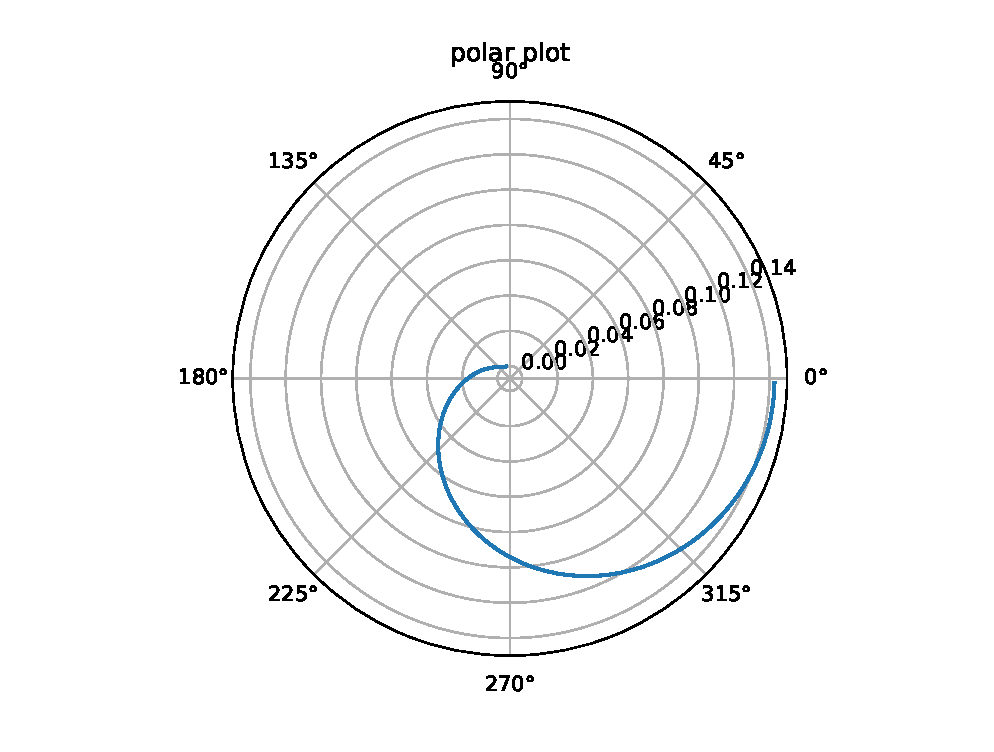
\includegraphics[width=\columnwidth]{polar.eps}
  \label{fig:polarplot}
\end{figure}

The following python code generates the polar plot below: 
\begin{lstlisting}
codes/ee18btech11033.py
\end{lstlisting}
\item How to tell about the stability of a closed loop system based on the polar plot?

\solution
The polar plots are for open loop transfer function,hence the reference point for determining stability is shifted to (-1,0).
\begin{description}[font=$\bullet$~\normalfont\scshape\color{red!50!black}]

\item If (-1,0) is to the left of the polar plot then the closed loop system is stable.
\item If (-1,0) is on the right side of the polar plot then the closed loop system is unstable.
\item If t(-1,0) is on the polar plot then the closed loop system is marginally stable.
\end{description}
\end{enumerate}
